% --------------------------------------------------------------
% This is all preamble stuff that you don't have to worry about.
% Head down to where it says "Start here"
% --------------------------------------------------------------

\documentclass[12pt]{article}

\usepackage[margin=1in]{geometry}
\usepackage{times}
\usepackage{amsmath,amsthm,amssymb}
\usepackage{caption}
\usepackage{graphicx,subfigure}
\usepackage{listings}
\usepackage{url}

\newcommand{\N}{\mathbb{N}}
\newcommand{\Gauss}{\mathcal{N}}
\newcommand{\Z}{\mathbb{Z}}
\newcommand{\E}{\mathbb{E}}
\newcommand{\R}{\mathbb{R}}
\newcommand{\p}{{\bf p}}
\newcommand{\1}{\mathbf{1}}

% \linespread{0}

\newenvironment{theorem}[2][Theorem]{\begin{trivlist}
\item[\hskip \labelsep {\bfseries #1}\hskip \labelsep {\bfseries #2.}]}{\end{trivlist}}
\newenvironment{lemma}[2][Lemma]{\begin{trivlist}
\item[\hskip \labelsep {\bfseries #1}\hskip \labelsep {\bfseries #2.}]}{\end{trivlist}}
\newenvironment{claim}[2][Claim]{\begin{trivlist}
\item[\hskip \labelsep {\bfseries #1}\hskip \labelsep {\bfseries #2.}]}{\end{trivlist}}
\newenvironment{exercise}[2][Exercise]{\begin{trivlist}
\item[\hskip \labelsep {\bfseries #1}\hskip \labelsep {\bfseries #2.}]}{\end{trivlist}}
\newenvironment{problem}[2][Problem]{\begin{trivlist}
\item[\hskip \labelsep {\bfseries #1}\hskip \labelsep {\bfseries #2.}]}{\end{trivlist}}
\newenvironment{question}[2][Question]{\begin{trivlist}
\item[\hskip \labelsep {\bfseries #1}\hskip \labelsep {\bfseries #2.}]}{\end{trivlist}}
\newenvironment{corollary}[2][Corollary]{\begin{trivlist}
\item[\hskip \labelsep {\bfseries #1}\hskip \labelsep {\bfseries #2.}]}{\end{trivlist}}

\begin{document}
{\raggedright

% --------------------------------------------------------------
%                         Start here
% --------------------------------------------------------------

\title{ECE 544NA HW5}%replace X with the appropriate number
\author{Jiaqi Mu~jiaqimu2 \\
% collaborating with Hongyu Gong~hgong6 \\
[8pt]%replace with your name
Department of Electrical and Computer Engineering} %if necessary, replace with your course title

\maketitle

\section{TensorFlow}
In this portion of the assignment, you will use a vanilla RNN and a LSTM to perform digit classification on the MNIST dataset.

\begin{itemize}
  \item {\bf Setting 1 (Sequence of Pixels):} It is assumed that each $28\times 28$ image, $x$, in the MNIST dataset is a sequence of single pixels, $x(1)$, ..., $x(784)$, where $x(t)$ is a single scalar value. The network reads one pixel at a time from the top left corner of the image to the bottem right of the image.
  \item {\bf Setting 2 (Sequence of Columns):} It is assumed that each $28\times 28$ image, $x$, in the MNIST dataset is a sequence of vectors, $x(1)$, ..., $x(28)$, where $x(t)$ is a $28\times 1$ vector representing one column in the image. The network reads one column at a time from left to right.
\end{itemize}

Train a basic (vanilla) RNN and a LSTM for each the two settings using a single layer RNN and LSRM with 100 hidden nodes. Perform classification on the last frame using cross entropy loss. 

\paragraph{Revelant Tensorflow Doc:} Tensorflow provides some API for recurrent neural network, please use the following:
\begin{itemize}
  \item {\tt tf.nn.rnn}: \url{https://github.com/tensorflow/tensorflow/blob/master/tensorflow/g3doc/api_docs/python/functions_and_classes/shard0/tf.nn.rnn.md}
  \item {\tt tf.nn.rnn\_cell}: \url{https://www.tensorflow.org/versions/r0.11/api_docs/python/rnn_cell.html#neural-network-rnn-cells}
\end{itemize}

\subsection{Methods} 
\begin{itemize}
  \item Describe the functions you wrote, and the overall structure of your code.
  \begin{proof}
  	We implemented RNN and LSTM in {\tt rnn.py} and {\tt lstm.py} respectively. The overall structures for both implementations are quite similar. Therefore, we simply describe the structure of a vanilla RNN. In LSTM, we simply replace the {\tt rnn\_cell} with a {\tt lstm\_cell}. In the RNN class, we implemented two functions for training and testing:
  	\begin{itemize}
  	 	\item {\tt fit}: to fit the data and learn the parameters from training data. In this module we build a graph structure using a RNN cell ({\tt tf.nn.rnn\_cell.BasicRNNCell}) and plug this in an existing RNN module.
      \item {\tt predict}: to predict labels for test data.
  	 \end{itemize} 
  \end{proof}
\end{itemize}

\subsection{Results}
\begin{itemize}
  \item Provide one figure with four subfigures, showing convergence plots of all four (2 settings, 2 models) classifiers (abscissa = training iteration, ordinate = training-corpus accuracy)
  \begin{proof}
    The figures are listed in Figure~\ref{fig:training}. Due to memory issue, we downsampled an image to $7\times 7$.
    \begin{figure}[htbp]
      \centering
      \subfigure[RNN-28*28]
      {
      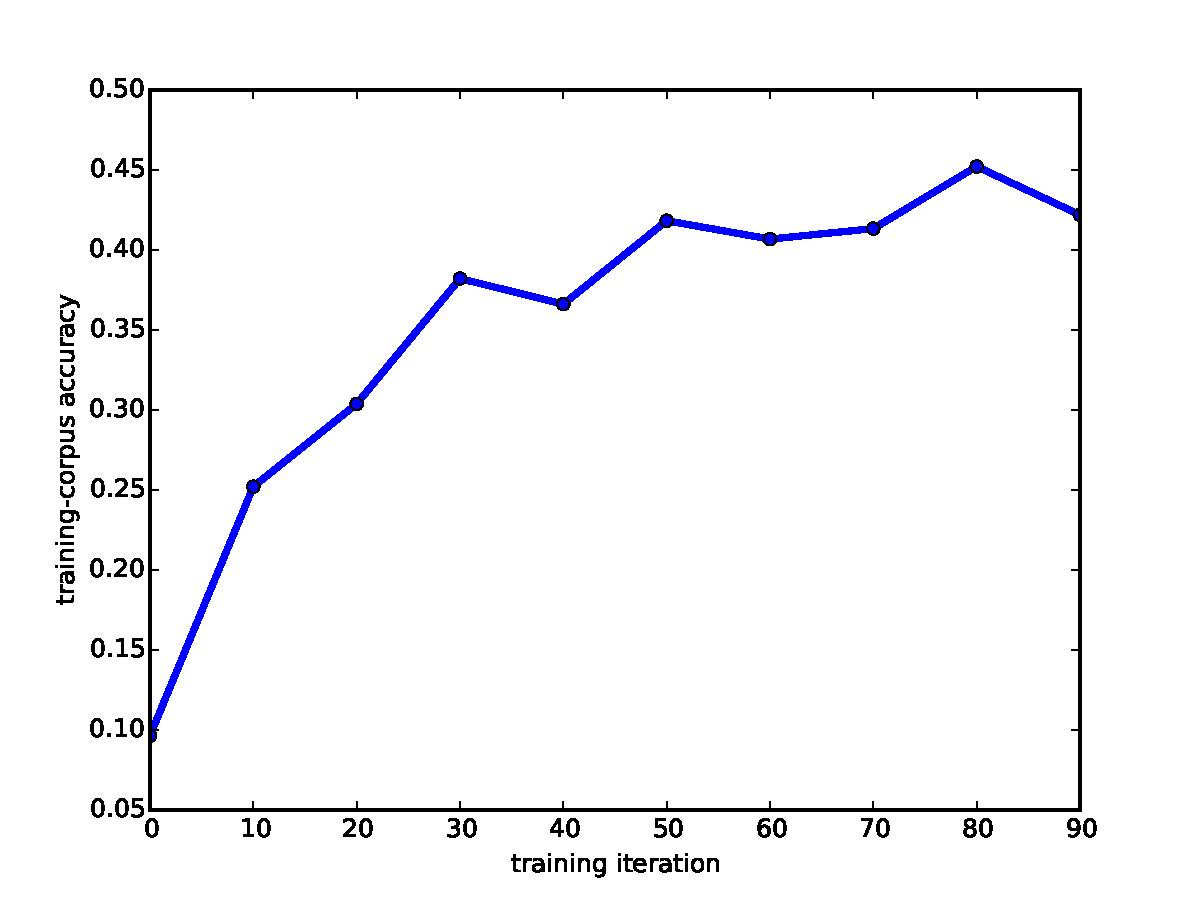
\includegraphics[width=0.4\textwidth]{../figures/RNN-28-28.pdf}
      }
      \subfigure[LSTM-28*28]
      {
      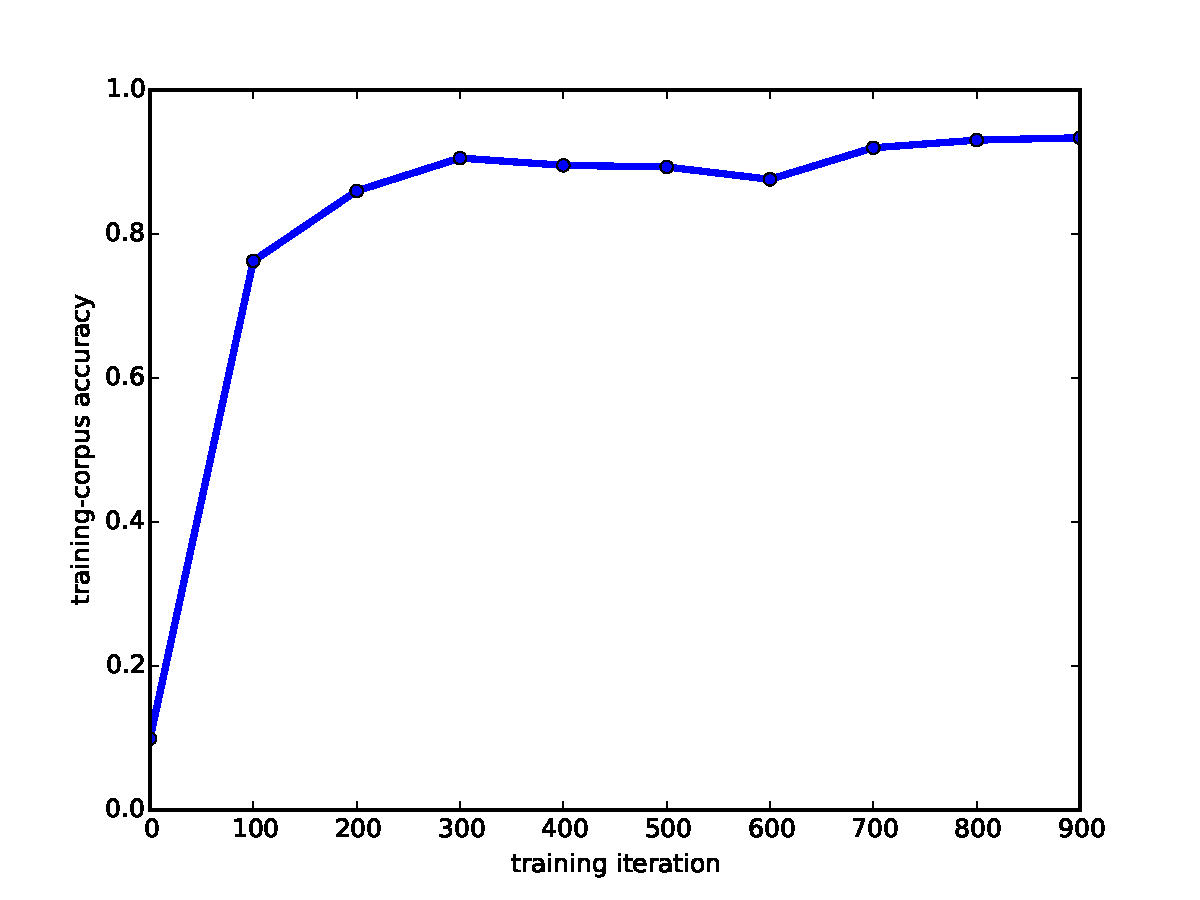
\includegraphics[width=0.4\textwidth]{../figures/LSTM-28-28.pdf}
      }
      \subfigure[RNN-49*1]
      {
      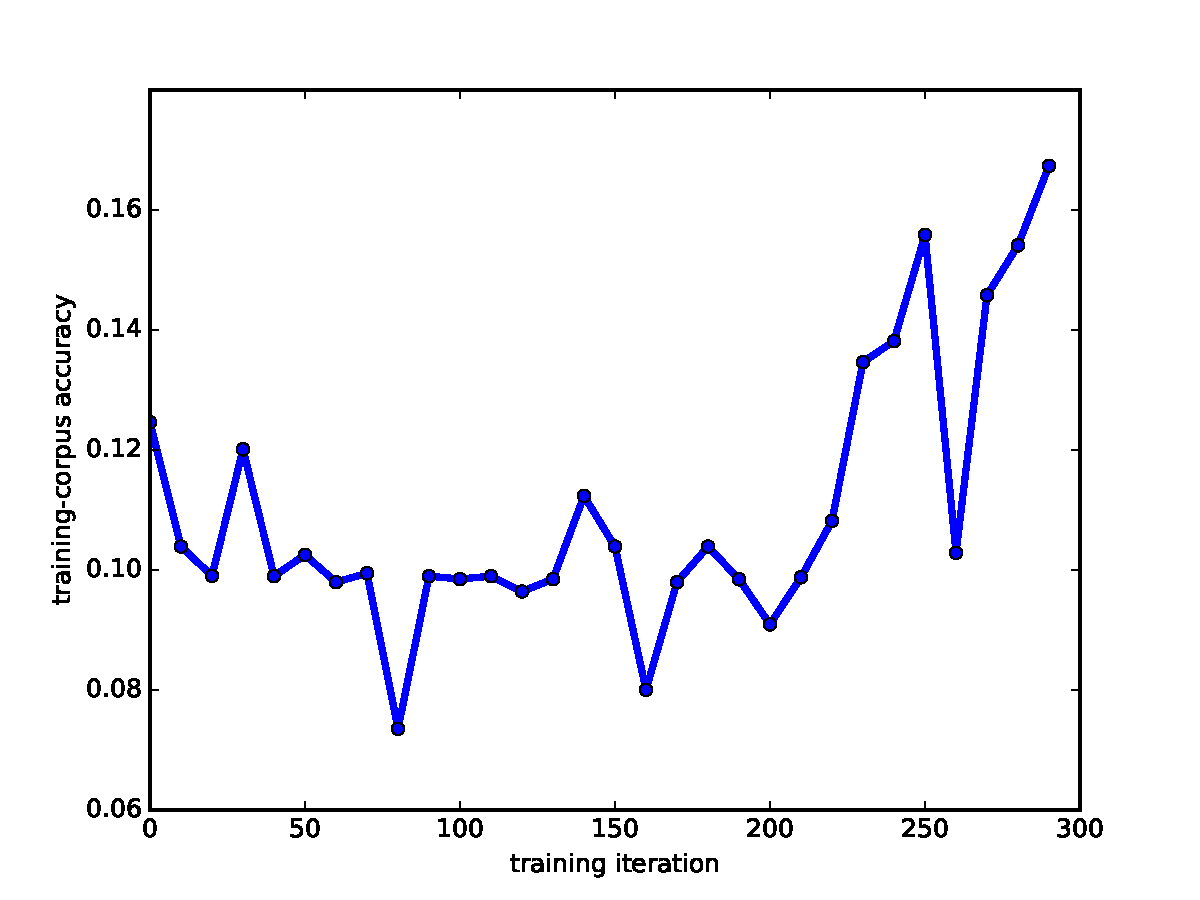
\includegraphics[width=0.4\textwidth]{../figures/RNN-49-1.pdf}
      }
      \subfigure[LSTM-49*1]
      {
      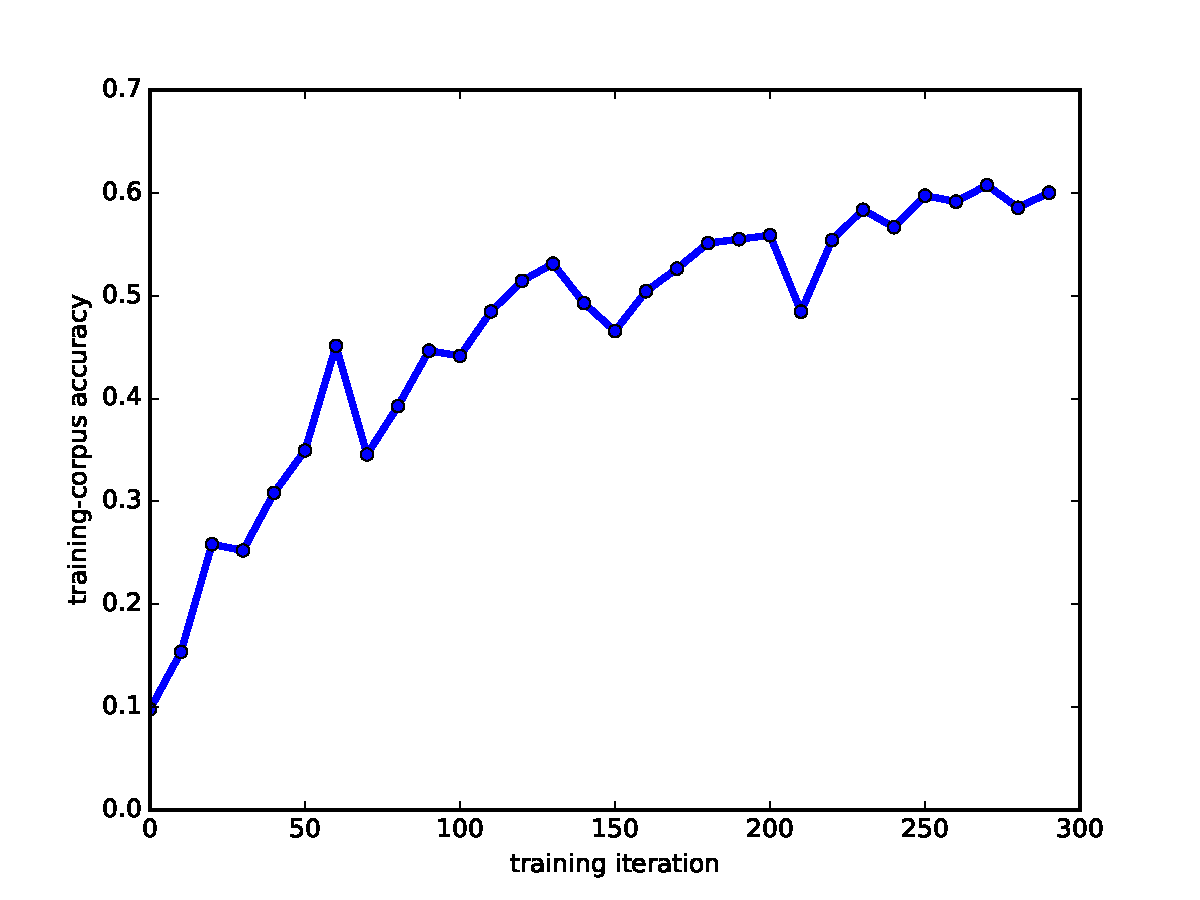
\includegraphics[width=0.4\textwidth]{../figures/LSTM-49-1.pdf}
      }
      \caption{Convergence plots. \label{fig:training}}
    \end{figure}
  \end{proof}
  \item Provide a table reporting the testing accuracies.
  \begin{proof}
    The accuracy is reported in Table~\ref{tb:test}.
    \begin{table}[htbp]
      \centering
      \begin{tabular}{r|c|c}
        \hline
        & 28*28 & 49*1 \\
        \hline
        RNN & 0.4586 & 0.1233 \\
        \hline
        LSTM & 0.9060 & 0.6183\\
        \hline
      \end{tabular}
      \caption{Accuracy.\label{tb:test}}
    \end{table}
  \end{proof}
\end{itemize}
\end{document}
